\documentclass[12pt]{article}
\usepackage{fullpage}
\usepackage{lscape}
\usepackage[top=2cm, bottom=4.5cm, left=2.5cm, right=2.5cm]{geometry}
\usepackage{amsmath,amsthm,amsfonts,amssymb,amscd}
\usepackage{lastpage}
\usepackage{enumerate}
\usepackage{fancyhdr}
\usepackage{mathrsfs}
\usepackage{graphicx}
\usepackage{subcaption}
\usepackage{listings}
\usepackage{hyperref}
\usepackage{titlesec}
\usepackage[T1]{fontenc}
\usepackage[utf8]{inputenc}
\usepackage{palatino}
\usepackage{booktabs}
\usepackage[dvipsnames]{xcolor}

\definecolor{grey}{gray}{0.6}

\newcommand{\SubItem}[1]{
    {\setlength\itemindent{15pt} \item[-] #1}
}

\newcommand\twoitems[2]{%
\item#1%
\hspace{20pt}%
\labelitemi
\hspace{\labelsep}#2
}

\setcounter{secnumdepth}{4}
\titleformat{\paragraph}
{\normalfont\normalsize\bfseries}{\theparagraph}{1em}{}
\titlespacing*{\paragraph}
{0pt}{3.25ex plus 1ex minus .2ex}{1.5ex plus .2ex}

\hypersetup{%
  colorlinks=true,
  linkcolor=blue,
  linkbordercolor={0 0 1}
}

\lstdefinestyle{C++}{
    language        = C++,
    frame           = lines, 
    basicstyle      = \footnotesize,
    keywordstyle    = \color{blue},
    stringstyle     = \color{olive},
    commentstyle    = \color{red}\ttfamily,
    breaklines      = true,
    tabsize         = 2
}

\setlength{\parindent}{0.0in}
\setlength{\parskip}{0.05in}

\newcommand\code{\url}
\newcommand\course{COMP0023}
\newcommand\hwnumber{}                   
\pagestyle{fancyplain}
\headheight 35pt
\lhead{\NetIDa}
\lhead{\course}                 
\chead{\textbf{\Large Assessment \hwnumber}}
\rhead{\today}
\lfoot{}
\cfoot{}
\rfoot{\small\thepage}
\headsep 1.5em

\graphicspath{{./images/}}

\begin{document}

\section{}

\subsection{Single Packet Perspective}

Each network layer will have its separate effort to detect and correct error regarding any bit errors or packet corruptions.

\subsubsection{Physical Layer L1}

Errors are detected on the link via Error Control Coding (ECC) and 
can potentially be further corrected by Forward Error Correction (FEC) methods. 

Slower Ethernet specifications (Fast Ethernet and Gigabit Ethernet) have limited error detection methods. For example, 8b/10b encoding used in Gigabit Ethernet does allow detecting single-bit errors, but no correction.

Later Ethernet developments include ECC methods and an FEC sublayer. 10GBASE-R PHYs(IEEE 802.3ap) uses the 64b/66b encoding, which provides at least a 4-bit hamming distance protection for all payload. It also specifies an optional RS-FEC(2112, 2080) sublayer using the Reed\textemdash Solomon error correction algorithm. Furthermore, higher symbol rate PHY links have much stronger FEC methods in place. 100G backplane PHY(IEEE 802.3ap) makes FEC mandatory in higher-bitrate or longer-distance connections.

A packet with fewer bit errors on a PHY with FEC can potentially be corrected. If no FEC or longer burst errors happened, the PHY might deem the received encoding invalid and discard the packet.

\subsubsection{Link Layer L2}

The link layer, notably Ethernet, employs an FCS appending to the end of the packet before the interframe gap. It is calculated using a CRC32 algorithm, transmitting in little-endian bit order. It is a powerful algorithm that detects:
\begin{itemize}
    \item All burst errors of length $\leq 31$
    \item All odd number of bit errors
    \item With high probability, burst errors of length $\geq 32$
\end{itemize}

Although there are several types of research regarding CRC-based error correction, it is still very rare in applicable hardware. Thus, we can assume that a faulty frame detected would be dropped.

\subsubsection{Network Layer L3 and Transport Layer L4}

In Internet Protocol version 4 (IPv4), its checksum is a 1's complement checksum operating upon the IP header only. Its primary purpose is to ensure correctness in a multi-hop environment. It aims to detect errors in intermediate machines, which could potentially alter the IP header during the packet transmission.

The TCP checksum is also 1's complement. It is enforced upon the TCP header, the TCP payload, and an IP pseudo-header. The IP pseudo-header includes the src/dst IP, TCP protocol number $\mathtt{0x06}$, and the IP size field from the lower level. It is meant to be an End-to-End (E2E) verification of the packet's integrity.

UDP checksum is optional upon UDP/IPv4 stack. Like TCP checksum, it is also a 1's complement of the header, payload and an IP pseudo-header. Contrary to IPv4, IPv6 does not have a checksum field. On a good note, no recalculation of checksum is needed upon forwarding packets. The L2 CRC and  L4 checksum would sufficiently check the L3 header. Hence, UDP/IPv6 has a mandatory checksum field.

1's complement is less powerful as it only guarantees single-bit error detection. It's primarily designed to work in a CPU-efficient (in bytes) and space-efficient (16 bits) way.

If the checksum detects an error in either (TCP/UDP)/(IPv4/IPv6), the packet would be dropped. In the rare case where L1-L4 ECC did not found the error, the corrupted packet would be sent to the upper layer.

\subsubsection{Summary}

In conclusion, the corrupted packet can either
\begin{itemize}
  \item gets corrected/dropped on PHY
  \item gets dropped on L2, L3, L4 if the checksum fails
  \item evades all checksums and gets passed on to the application
\end{itemize}

\subsection{End-To-End Perspective}

In the following discussions, we will divide each section into whether the corrupted bit is detected or not in ECCs of L1-L4.

\subsubsection{DNS transactions}

Upon typing \url{www.ucl.ac.uk} into the browser, the laptop would first query DNS to obtain the IP address. We assume the domain operates with DNS instead of DNSSEC.

\begin{itemize}
    \item Laptop looks up the DNS in cache. Since it's a new laptop, nothing would be found.
    \item Laptop sends a DNS request to a DNS server, usually a local/public DNS resolver.
    \item If found, the DNS reply containing \url{www.ucl.ac.uk}'s IP address would be replied.
    \item If not found, the DNS resolver would start resolving \url{www.ucl.ac.uk} from the root servers, all the way down to its authoritative nameservers (e.g. \url{dns-ns1.ucl.ac.uk}).
    \item Similarly, a DNS reply of \url{www.ucl.ac.uk} would be sent to the laptop.
\end{itemize}

\paragraph{Packet Error Detected}

The packet would most likely be discarded by a switch, router or server upon corruption. Then, the laptop browser would timeout on the query and resend it after a while. 

\paragraph{Packet Error Not Detected}

This rare case would result in either an invalid DNS query or a DNS query targetting a different domain. The common case would be an invalid DNS query. The name server or resolver shall detect this and drop this invalid DNS query. The rarer case would be the request reaching an entirely different authoritative server and getting either a \url{NXDOMAIN} reply or a reply on a different domain (e.g. \url{www.ual.ac.uk}). The laptop would found the response unrelated to its question. Hence, re-querying the DNS.

\subsubsection{HTTP transactions}

\url{www.ucl.ac.uk} shall be HTTP webpages (certainly not Gopher). Although UCL serves only HTTP/1.1, \url{www.ucl.ac.uk/} also includes content served by CDN through HTTP/3, optionally. It's notable that HTTP/3 is based on QUIC/UDP/IP stack, while HTTP/1.1 on a TCP/IP stack. Moreover, when serving HTTPS/1.1, there's a TLS layer in between HTTP and TCP. We limit the scope to HTTP/TCP/IP stack in this question.

\paragraph{Packet Error Detected}

The TCP establishment includes three handshakes. If the laptop's packet corrupted on the first SYN or the third ACK, the server would not respond. The laptop's RTX timer would run out and it resends the same packet.

If any laptop's packet gets corrupted during the transmission process, the laptop's RTX timer will timeout as the server ACK will not happen. The laptop would then attempt to retransmit until ACKed.

The TCP teardown is comprised of four handshakes. If the first FIN from the laptop gets corrupted, the server would not reply with an ACK. After the laptop's RTX timeout, it would resend FIN.

Suppose the fourth ACK (corresponding to server FIN) corrupts; the laptop would have already entered a TIME\_WAIT state, expecting to close the connection after 2 MSLs. However, the server would eventually reach RTX timeout as its FIN not ACKed. The server would retransmit a FIN to the laptop, reaching the laptop during TIME\_WAIT. The laptop will then retransmit ACK to the server and successfully close the connection.

\paragraph{Packet Error Not Detected}

In the rare case where the packet error is not detected, the serving application might receive a corrupted request. Typically, the HTTP request would be an invalid one. In the extreme case where the corrupted HTTP request is valid and contains a different URL, the server might respond with a 404 or with a wrong page. The server behaviour would be unpredictable in this case.


\newpage
\section{}

\renewcommand{\thesubsection}{\thesection.\alph{subsection}}

\subsection{}

\begin{figure}[h!]
  \makebox[\textwidth][c]{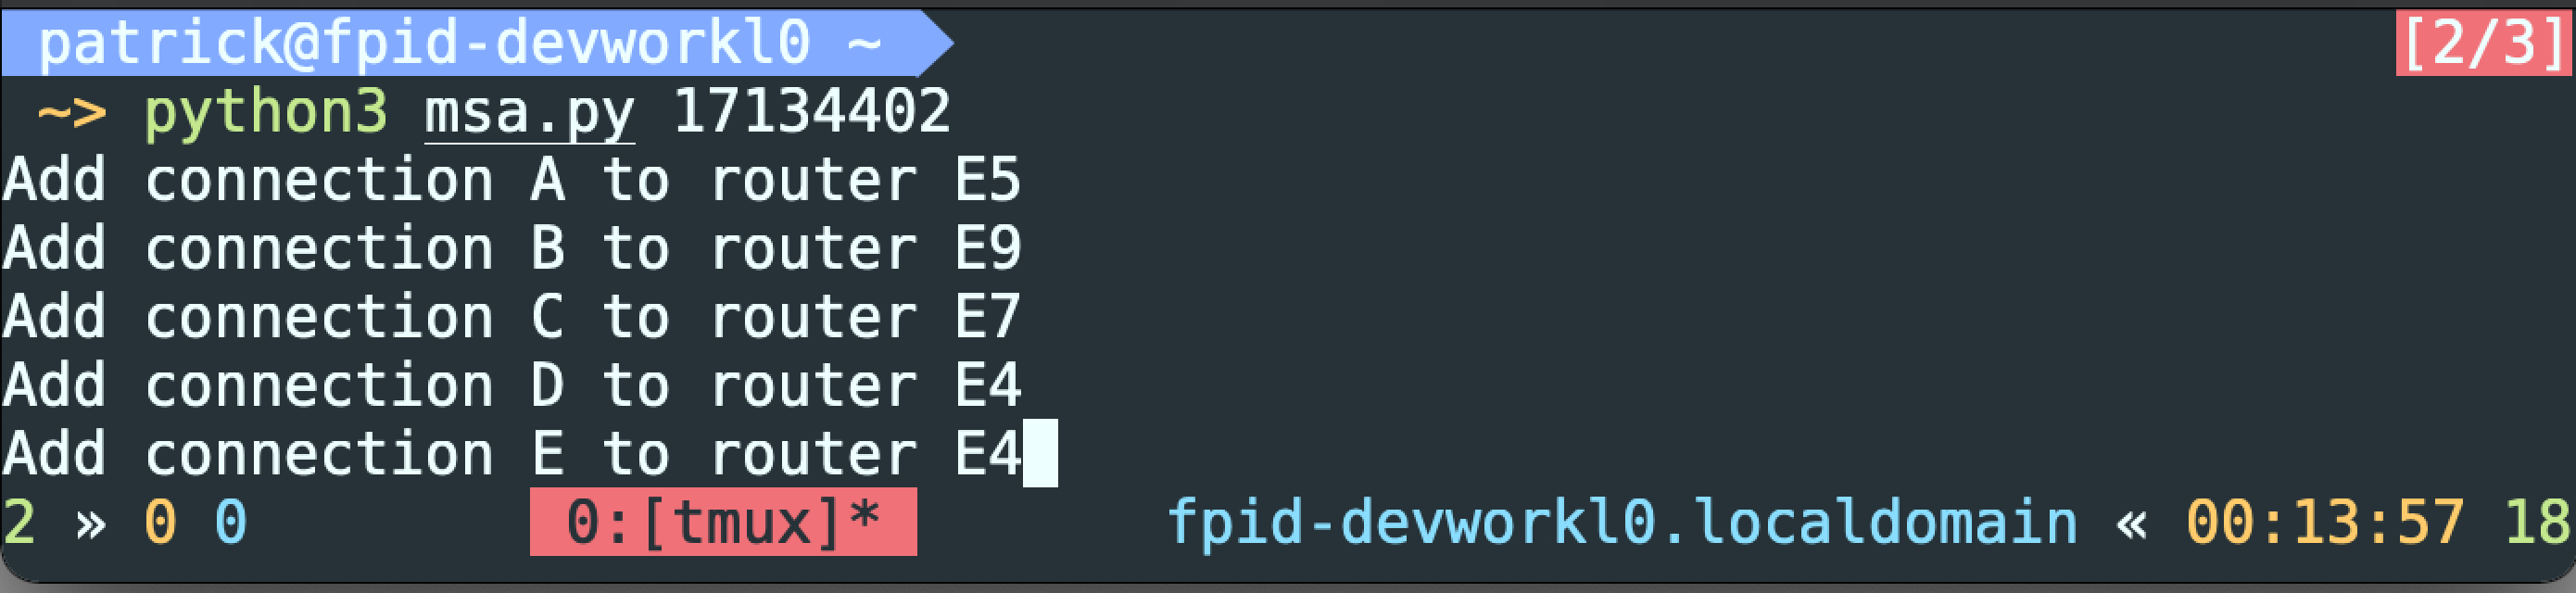
\includegraphics[width=\textwidth]{imgs/python-script-screenshot.png}}
  \caption{Python Script Screenshot}
  \label{fig:python-screenshot}
\end{figure}

\begin{figure}[h!]
  \makebox[\textwidth][c]{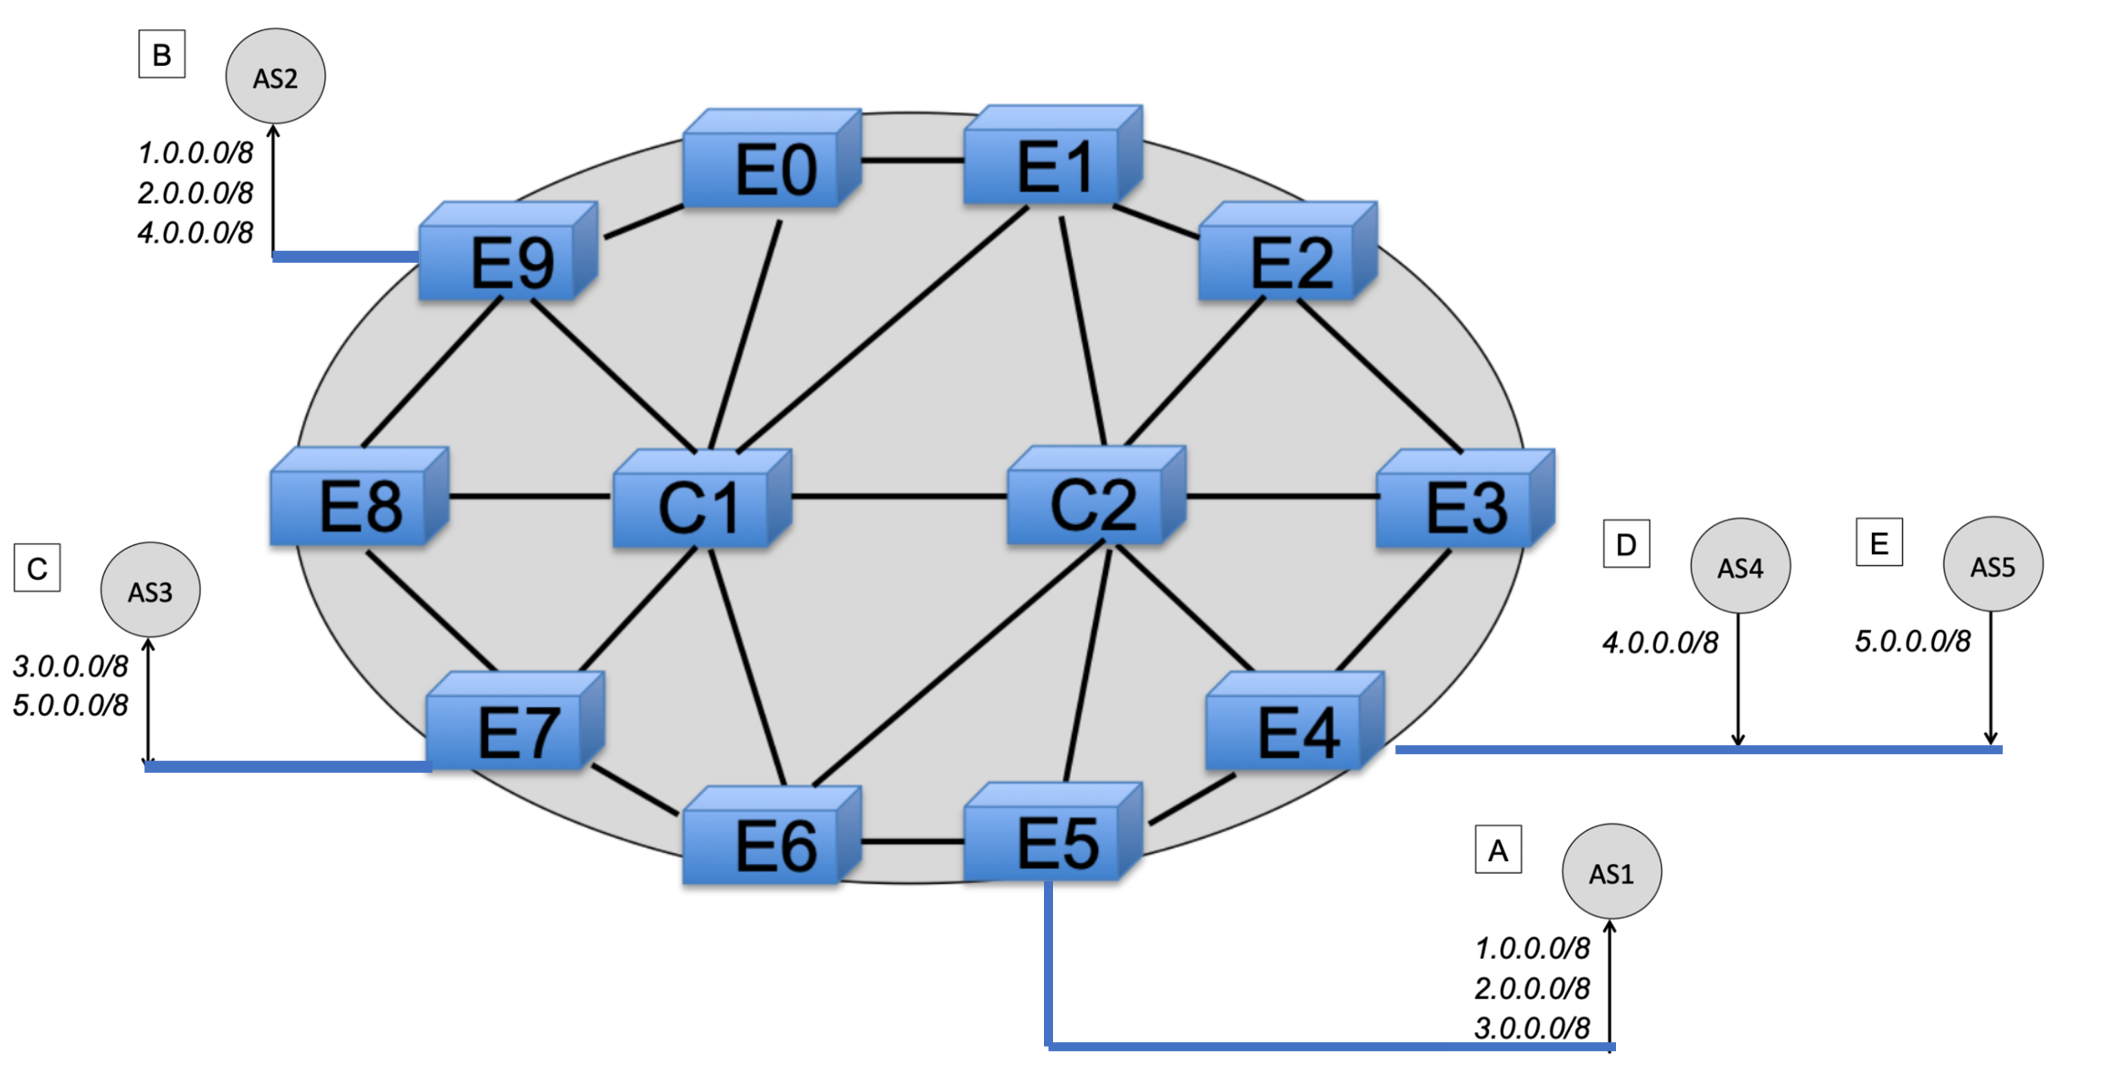
\includegraphics[width=1.1\textwidth]{imgs/topology.png}}
  \caption{Topology}
  \label{fig:topology}
\end{figure}

\newpage
\subsection{}

We constraint the scope to BGP and IGPs mentioned in COMP0023 lectures.

Consider two paths destined to 1.0.0.0/8:
\begin{itemize}
    \twoitems{E9 \textrightarrow{} C1 \textrightarrow{} C2 \textrightarrow{} E5}{E5 \textrightarrow{} C2 \textrightarrow{} C1 \textrightarrow{} E9}
\end{itemize}

We will prove below that these two paths are mutually incompatible.

\subsubsection{Assume E9 \textrightarrow{} C1 \textrightarrow{} C2 \textrightarrow{} E5 (1.0.0.0/8) is configured}

Referring to BGP routing priority, we look at all possibilities for this route to exist:
\begin{itemize}
    \item LOCAL PREF (LP): E9 and E5 are BGP routers connecting to a neighbouring provider AS1 and AS2. They shall have the same LP.
    \item \textbf{AS-PATH: If AS-PATH to 1.0.0.0/8 is longer for AS2 than AS1, E9 would be forced to route to egress E5 to AS1.}
    \item \textcolor{grey}{ORIGIN, MED: IGP is used for ORIGIN, and MED is invalid as E5 connects to AS1 and E9 connects to AS2}
    \item eBGP \textgreater{} iBGP: E9 and E5 are both routers with egress connection to 1.0.0.0/8.
    \item \textbf{IGP distance: Tie-breaker, E9 \textrightarrow{} AS2 (1.0.0.0/8) is always shorter than E9 \textrightarrow{} C1 \textrightarrow{} C2 \textrightarrow{} E5 \textrightarrow{} AS1 (1.0.0.0/8)}
\end{itemize}

The only explanation would be the AS-PATH assumption above is valid. Then, E5 \textrightarrow{} C2 \textrightarrow{} C1 \textrightarrow{} E9 (1.0.0.0/8) would be invalid. Instead, E5 \textrightarrow{} AS2 shall be the egress point of 1.0.0.0/8 within AS Y.

\subsubsection{Assume E5 \textrightarrow{} C2 \textrightarrow{} C1 \textrightarrow{} E9 (1.0.0.0/8) is configured}

Vice versa, the only underlying reasoning now would be: AS-PATH to $1.0.0.0/8$ is longer for AS1 than AS2. Thus, E9 shall be the only egress point of 1.0.0.0/8 within AS Y. E9 \textrightarrow{} C1 \textrightarrow{} C2 \textrightarrow{} E5 (1.0.0.0/8) would not happen.

\subsection{}

In this section, we will be discussing changes made to BGP priority and IGP. These changes will only affect intra-domain routing.

In order to allow both paths to be configured simultaneously, we would have to enforce a routing protocol that does load balancing and allows multiple BGP egress point of the same IP address prefix. Therefore, we propose the following changes:

\begin{itemize}
    \item If no loop is detected through AS-PATH, consider both egress routes viable.
    \item Incorporate multiple egress points of a certain IP address prefix within the routing table. Each egress point is given a score based on the AS-PATH; the longer the AS-PATH, the lower the score.
    \item Consider a novel packet (either originated within the AS, or came into the AS through a border router):
    \SubItem{Destined to a foreign IP prefix, the first router that sees the packet should use a probability generator with weight (score) to tag the packet's egress point.}
    \SubItem{Destined to an IP within the AS, the first router would tag the packet with the destination router.}
    \item Within the AS, only route packets based on router tag and disregard IP prefix.
    \item On the packet reaching the internal destination, or exiting the AS, remove the packet destination tag.
\end{itemize}

For example, in this particular topology, we assume E5\textrightarrow{}AS1\textrightarrow{}1.0.0.0/8 has AS-PATH length of 1, while E9\textrightarrow{}AS2\textrightarrow{}1.0.0.0/8 has length of 2. The new protocol would then deem both routers valid egress point of 1.0.0.0/8, although E5 has a 2-times higher probability of being tagged as the destination.

The calculation of probabilities can be synthesised through the propagation of iBGP within the network, similar to that of Link-State IGP flooding. Once all routers reach a consensus on the routing table probability distribution, we can start routing the packets. For instance, consider a packet destined to 1.0.0.0/8 originates at C1, C1 uses a random generator with weight to decide this specific packet shall go to \textbf{E9} instead of \textcolor{grey}{E5}. The packet would then follow AS's IGP routing to E9 and gets forwarded to AS2. The total amount of packets egressing through E5 and E9 (2:1) shall be roughly inversely proportional to the AS-PATH ratio (1:2).

The reason why we added a destination tag upon reaching the first router in the system is to avoid looping. Consider a packet originating in C1 and going to 1.0.0.0/8, C1 randomised a path of C1\textrightarrow{}C2\textrightarrow{}E5, hence forwarding to C2. C2 then randomised, with lower probability but still likely, C2\textrightarrow{}C1\textrightarrow{}E9, and delivered it back to C1. This creates a loop we would like to avoid. Therefore, we enforce a concrete destination once the packet enters the routing system, hence the tagging.

Compared to the traditional BGP, this approach brings a more balanced traffic load to the AS internally and neighbouring AS. Consider a spike in traffic heading towards 1.0.0.0/8: With the conventional BGP, traffic would be congested at E9/E5, and that single router limits the 1.0.0.0/8 traffic output capacity of the whole AS. Now that the same IP prefix can have multiple egress points, a proportion of the congested traffic can be diverted to other edge routers, balancing the load.

However, this approach introduces unwanted overhead in tagging and untagging packets upon entering and exiting the AS routing system. This could potentially slow down packet forwarding in switches. In order to facilitate this tagging approach within the AS, its owners might need to purchase advanced network equipment that supports this type of custom-configured routing protocols, incurring extra cost.

In all, this approach takes the idea from multi-path BGP and Ethernet VLAN tagging to achieve the originally incompatible paths simultaneously. The benefit of balanced load under bursty traffic comes with the trade-off the extra randomisation and tagging overhead, as well as the requirement of more customisable routers.

\end{document}